\chapter{Descrizione del Progetto}
\label{cap:descrizione}

Questo capitolo introduce i preliminari tecnici e illustra il problema affrontato. La sezione \ref{Scenario} è dedicata alla descrizione del contesto tecnologico mentre la sezione \ref{Problema} analizza le problematiche affrontate nello studio. 

\section{Scenario Tecnico}
\label{Scenario}
\subsection{Modello ISO/OSI e Protocolli di Rete}
~\\
\indent I protocolli di rete sono una componente essenziale per la comunicazione tra dispositivi su una rete. 
Definiscono le regole e gli standard per il trasferimento dei dati, assicurando che le informazioni vengano trasmesse e comprese correttamente.
Per facilitare la comprensione e l'organizzazione di questi protocolli, è utile fare riferimento al modello \emph{ISO/OSI (Open Systems Interconnection)}.
Questo standard architetturale suddivide i protocolli in sette livelli distinti elencati in Figura \ref{iso-osi}, ognuno con un compito specifico.
\begin{figure}[!h]
    \centering
    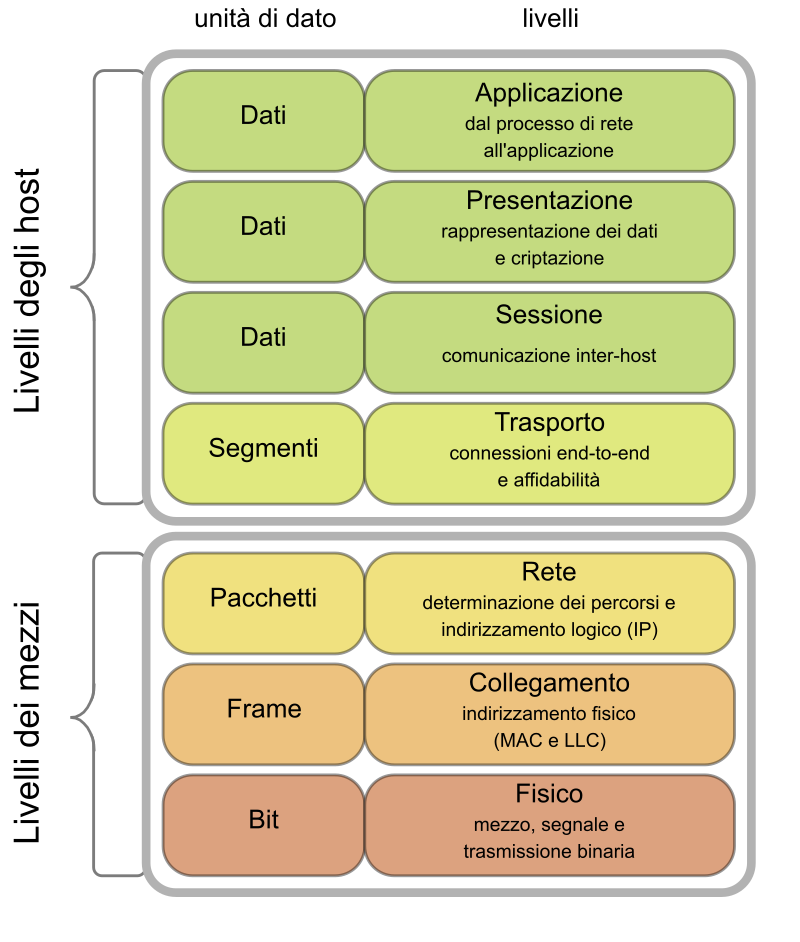
\includegraphics[width=0.5\columnwidth]{descrizione/tcp/iso}
    \caption{\emph{Raffigurazione del modello ISO/OSI}}
    \label{iso-osi}
\end{figure}
Di seguito, viene riportata una descrizione del ruolo di ogni livello: 
\begin{enumerate}
    \item \textbf{Livello Fisico}: Il livello fisico si occupa della trasmissione effettiva dei bit attraverso il mezzo fisico della rete, in questo livello lavorano i \emph{modem} e gli \emph{hub}. 
    \item \textbf{Livello Data Link}: Il livello \emph{data link} gestisce la comunicazione tra dispositivi sulla stessa rete fisica. Si occupa di garantire che il trasferimento mediante il livello fisico sia affidabile effettuando un controllo degli errori. A questo livello operano \emph{switch} e i \emph{bridge}.
    \item \textbf{Livello Rete}: Il livello di rete gestisce l'instradamento ottimale dei pacchetti di dati tra reti diverse. Il protocollo principale che opera a questo livello è l'\emph{Internet Protocol (IP)}. 
    \item \textbf{Livello Trasporto}: Il livello di trasporto controlla il flusso di dati e gestisce la segmentazione dei pacchetti. Garantisce la corretta trasmissione delle informazioni. I protocolli principali includono \emph{TCP} e \emph{UDP}.
    \item \textbf{Livello Sessione}: Il livello di sessione gestisce l'apertura, il controllo e la chiusura delle sessioni di comunicazione. 
    \item \textbf{Livello Presentazione}: Il livello di presentazione è responsabile della traduzione e della formattazione dei dati tra il formato utilizzato dalle applicazioni a quello della rete. Protocolli come \emph{Secure Sockets Layer (SSL)} e \emph{Transport Layer Security (TLS)} ne fanno parte.
    \item \textbf{Livello Applicazione}: Il livello di applicazione fornisce un insieme di protocolli che operano a stretto contatto con le applicazioni. Protocolli come \emph{HTTP},\emph{FTP} e \emph{SMTP} ne fanno parte.

\end{enumerate}


\subsection{Protocolli di Trasporto Tradizionali}
~\\
\indent Nel panorama dei \emph{protocolli di rete}, i \emph{protocolli di trasporto} \emph{TCP (Transmission Control Protocol)}  e \emph{UDP (User Datagram Protocol)} hanno svolto e svolgono tutt'ora un ruolo fondamentale sin dalla nascita di Internet.
Questi protocolli sono stati la spina dorsale delle comunicazioni per decenni, supportando una vasta gamma di servizi e applicazioni.\\
Pur appartenendo alla stessa famiglia di protocolli, \emph{TCP} e\emph{UDP} sono stati concepiti con caratteristiche e obbiettivi distinti e vengono impiegati in base alle specifiche esigenze applicative.
In particolare \emph{TCP}, con la sua affidabilità e il suo controllo di flusso, ha svolto un ruolo fondamentale nelle comunicazioni che richiedevano l'integrità dei dati, mentre \emph{UDP} ha trovato il suo spazio nei servizi che privilegiavano la velocità rispetto all'affidabilità. 
Tuttavia, con l'evoluzione delle nuove tecnologie, le limitazioni di questi protocolli sono diventate sempre più evidenti. Nella concezione di base di \emph{TCP} e \emph{UDP}, ideata agli inizi del 1970, non erano state previste le sfide delle reti moderne, 
caratterizzate da:  
\begin{itemize}
    \item Connessioni mobili e variabili;
    
    \item Necessità di ridurre la latenza;
    
    \item Proliferazione di dispositivi \emph{IoT}\footnote{\gls{IoT}};
     
    \item Requisiti di sicurezza sempre più vincolanti.
\end{itemize}

\noindent Queste nuove sfide hanno evidenziato una serie di problematiche nei protocolli. La consapevolezza di questi limiti ha portato alla ricerca di nuove soluzioni, cercando di superare le inefficienze pur mantenendo i punti di forza dei protocolli tradizionali.
Questi studi hanno portato alla creazione di nuovi protocolli come \emph{QUIC} ed a estensioni come \emph{MPTCP}, che cercano di superare le limitazioni di \emph{TCP} e \emph{UDP} per far fronte alle sfide del mondo moderno, offrendo prestazioni migliori, maggiore sicurezza e flessibilità.
\subsubsection{TCP (Transmission Control Protocol)}
~\\
% Fonte https://www.ietf.org/rfc/rfc793.txt %
\indent Il \emph{Transmission Control Protocol (TCP)} è uno dei protocolli cardine su cui si basa la comunicazione su Internet. 
Dato il suo ruolo e la vasta gamma di funzioni che offre, un'analisi completa del suo funzionamento e della sua costituzione richiederebbe un'analisi approfondità che va oltre lo scopo di questa tesi.
Pertanto, in questa sezione, ci si concentrerà solo su alcuni aspetti specifici del \emph{TCP} che sono fondamentali per la comprensione del problema affrontato in questa tesi. 
In particolare, verranno esaminate nel dettaglio :
\begin{itemize}
    \item Caratteristiche principali di una connessione \emph{TCP};
    
    \item Il processo di \emph{Handshake}\footnote{\gls{Handshake}};
    
    \item Il meccanismo di Ritrasmissione;
    
    \item I metodi utilizzati per garantire la sicurezza dei dati.
\end{itemize}

\paragraph{\textit{Caratteristiche principali}}
\noindent Il \emph{Transmission Control Protocol} si distingue come un protocollo orientato alla connessione. Questa sua caratteristica significa che, prima di qualsiasi scambio di dati, deve essere stabilita una connessione dedicata tra il \emph{client}\footnote{\gls{client}} e il \emph{server}\footnote{\gls{server}}.
Tale peculiarità è alla base di molte delle sue funzionalità avanzate, tra cui:
\begin{description}
    \item[Affidabilità] Garantisce che i dati trasmessi vengano ricevuti correttamente.

    \item[Controllo di Errore] Implementa un sistema di verifica della integrità dei dati tramite il meccanismo di \emph{checksum}\footnote{\gls{checksum}}.
    
    \item[Controllo di Flusso e Congestione] Utilizza il sistema delle \emph{sliding window}\footnote{\gls{sliding window}} per ottimizzare il flusso di dati e diminuire il numero di segmenti ritrasmessi in caso di situazione di congestione.
\end{description}

\noindent Queste funzionalità si riflettono sulla struttura stessa di un segmento \emph{TCP}, come si può vedere nella Figura \ref{fig}. 
Di seguito, è riportata la descrizione di alcune sezioni di interesse per il problema analizzato:

\begin{itemize}
\item \textit{\textbf{Source Port - Destination Port}}: Identificano rispettivamente il numero della porta di origine e destinazione.
\item \textit{\textbf{Sequence Number}}: Indica la posizione del primo segmento \emph{TCP} all'interno del flusso a partire dall'\emph{ISN}\footnote{\gls{ISN}}, deciso durante la inizializzazione della connessione.
\item \textit{\textbf{Acknowledgement Number}}: Se il \emph{control bits ACK} è presente questo campo contiene il valore del prossimo \emph{sequence number} che il ricevente del segmento si aspetta di ricevere.
\item \textit{\textbf{Control Bits}}: Sono dei bit utilizzati per il controllo del protocollo. 
\begin{itemize}
    \item \textit{\textbf{URG}}: Se impostato a 1 indica la presenza di dati urgenti.
    \item \textit{\textbf{ACK}}: Se impostato a 1 indica che l'\emph{acknowledgement number}\footnote{\gls{acknowledgements}} è valido.
    \item \textit{\textbf{PSH}}: Se impostato a 1 indica che i dati devono essere elaborati dai livelli superiori.
    \item \textit{\textbf{RST}}: Se impostato a 1 indica che la connessione non è più valida.
    \item \textit{\textbf{SYN}}: Se impostato a 1 indica che il mittente vuole stabilire una connessione \emph{TCP}.
    \item \textit{\textbf{FIN}}: Se impostato a 1 indica che il mittente vuole terminare la connessione \emph{TCP}.
\end{itemize}
\item \textit{\textbf{Checksum}}: Valore utilizzato per verificare la validità del segmento. Si ottiene facendo il complemento a uno della somma complementare a uno a 16 bit dell'\emph{header} e del \emph{payload}.
\item \textit{\textbf{Data}}: Contiene l'informazione da trasmettere.
\end{itemize}

\begin{figure}[!h]
\centering
\begin{BVerbatim}
 0                   1                   2                   3   
 0 1 2 3 4 5 6 7 8 9 0 1 2 3 4 5 6 7 8 9 0 1 2 3 4 5 6 7 8 9 0 1 
+-+-+-+-+-+-+-+-+-+-+-+-+-+-+-+-+-+-+-+-+-+-+-+-+-+-+-+-+-+-+-+-+
|          Source Port          |       Destination Port        |
+-+-+-+-+-+-+-+-+-+-+-+-+-+-+-+-+-+-+-+-+-+-+-+-+-+-+-+-+-+-+-+-+
|                        Sequence Number                        |
+-+-+-+-+-+-+-+-+-+-+-+-+-+-+-+-+-+-+-+-+-+-+-+-+-+-+-+-+-+-+-+-+
|                    Acknowledgment Number                      |
+-+-+-+-+-+-+-+-+-+-+-+-+-+-+-+-+-+-+-+-+-+-+-+-+-+-+-+-+-+-+-+-+
|  Data |           |U|A|P|R|S|F|                               |
| Offset| Reserved  |R|C|S|S|Y|I|            Window             |
|       |           |G|K|H|T|N|N|                               |
+-+-+-+-+-+-+-+-+-+-+-+-+-+-+-+-+-+-+-+-+-+-+-+-+-+-+-+-+-+-+-+-+
|           Checksum            |         Urgent Pointer        |
+-+-+-+-+-+-+-+-+-+-+-+-+-+-+-+-+-+-+-+-+-+-+-+-+-+-+-+-+-+-+-+-+
|                    Options                    |    Padding    |
+-+-+-+-+-+-+-+-+-+-+-+-+-+-+-+-+-+-+-+-+-+-+-+-+-+-+-+-+-+-+-+-+
|                             data                              |
+-+-+-+-+-+-+-+-+-+-+-+-+-+-+-+-+-+-+-+-+-+-+-+-+-+-+-+-+-+-+-+-+
           \end{BVerbatim}
\caption{\textit{Composizione di un segmento TCP}}
\label{fig}
\end{figure}

\noindent Una connessione \emph{TCP} è dunque identificata univocamente da quattro elementi:

\begin{center}
    \small
    $[\text{Indirizzo IP sorgente}, \text{Porta sorgente}] \leftrightarrow [\text{Indirizzo IP destinazione}, \text{Porta destinazione}]$
\end{center}

\noindent Questa struttura offre diversi vantaggi. Ad esempio, permette ad un singolo \emph{server} di accettare più connessioni contemporaneamente da diversi \emph{client}, e viceversa. 
Inoltre garantisce l'unicità di ogni connessione all'interno della rete.
\\
Ciononostante, questa rigida definzione di una connessione presenta delle limitazioni significative, in quanto qualsiasi modifica a uno dei quattro elementi, come un cambio di porta o una migrazione dell'indirizzo IP, comporta la chiusura della connessione esistente.
Questa limitazione diventa ancora più rilevante nel contesto delle comunicazioni moderne, dove situazioni di \emph{multihoming}\footnote{\gls{multihoming}} e cambi frequenti di indirizzo IP sono sempre più comuni \cite{site:tcp}. 
\\
\\
Questa problematica, come verrà sottolineato nelle prossime sezioni, è alla base di soluzioni come \emph{MPTCP} e viene affrontata in modo indiretto anche in \emph{QUIC}.

\paragraph{\textit{Handshake}}
% https://it.wikipedia.org/wiki/Round_Trip_Time

\noindent Uno dei punti cardine del \emph{TCP} è la necessità di stabilire una connessione prima di qualsiasi scambio di dati. Questo processo, noto come \emph{three-way handshake} ("stretta di mano in tre passaggi"), richiede lo scambio di tre messaggi tra \emph{server} e \emph{client}. La Figura \ref{handshake} illustra questo procedimento.

\begin{figure}[!h]
    \centering
    \begin{minipage}{0.48\textwidth}
        \centering
        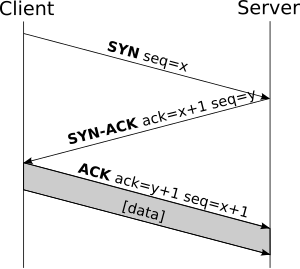
\includegraphics[width=0.75\columnwidth]{descrizione/tcp/three-way-handshake}
        \caption{\emph{Processo three-way handshake in TCP}}
        \label{handshake}
    \end{minipage}
    \hfill
    \begin{minipage}{0.48\textwidth}
        \centering
        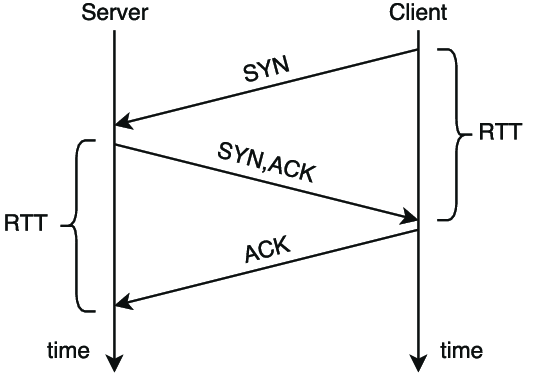
\includegraphics[width=0.90\columnwidth]{descrizione/tcp/rtt-handshake}
        \caption{\emph{Definizione di RTT (Round Trip Time)}}
        \label{rtt}
    \end{minipage}
\end{figure}

\noindent I passaggi coinvolti in questo processo sono i seguenti: 

\begin{enumerate}
    \item \textbf{Client invia un segmento SYN al Server}: Il segmento ha il campo \emph{SYN} impostato a 1 e il suo \emph{sequence number} contiene il valore x che rappresenta l'\emph{ISN (Initial Sequence Number)} del \emph{Client}.
    \item \textbf{Server invia un segmento SYN/ACK al Client}: Il \emph{server} risponde con un segmento i cui campi \emph{SYN} e \emph{ACK} sono impostati a 1. Il suo \emph{sequence number} contiene un nuovo valore y che specifica l'\emph{ISN} del \emph{server} e il campo \emph{Acknowledgement number} contiene il valore \emph{x+1} del \emph{client}.
    \item \textbf{Client invia un segmento ACK al Server}: Il \emph{client} risponde inviando un segmento il cui campo \emph{ACK} è impostato a 1 e l'\emph{acknowledgement number} è dato da \emph{y+1}.
\end{enumerate}

\noindent Oltre a stabilire la connessione, l'\emph{handshake} riveste un ruolo fondamentale in vari aspetti della comunicazione \emph{TCP}.
Non solo permette di sincronizzare i \emph{sequence number}, ma fornisce anche una base inziale per misurare il \emph{Round Trip Time (RTT)}\footnote{\gls{RTT}} (Figura \ref{rtt}), che rappresenta il tempo totale necessario per un pacchetto di dati per viaggiare dal mittente al destinatario e ritorno. La misurazione di questo valore è essenziale per ottimizzare il controllo di flusso e la gestione della congestione della rete \cite{site:tcp}.

\paragraph{\textit{Ritrasmissioni}}

\noindent In seguito viene descritto brevemente il meccanismo di ritrasmissione utilizzato da \emph{TCP}, che risulta necessario per comprendere alcuni concetti della tesi.
\\\\
\noindent Il \emph{TCP} è un protocollo progettato per garantire l'affidabilità nella comunicazione dei dati. Durante la trasmissione, i pacchetti possono venire persi o essere danneggiati a causa di vari fattori, come congestione della rete, interferenze o errori \emph{hardware}.
La ritrasmissione dei questi segmenti è uno dei meccanismi chiave per garantire l'integrità dei dati. Questo processo si basa sulla logica degli \emph{acknowledgements}. Quando un segmento viene inviato, il mittente attende una conferma di ricezione (\emph{ACK}) dal destinatario. Se questa conferma non viene ricevuta entro un determinato intervallo di tempo, chiamato \emph{Retransmission TimeOut (RTO)}\footnote{\gls{RTO}}, il mittente assume che il segmento sia stato perso e lo ritrasmette.
Il calcolo del RTO è dinamico e dipende fortemente dal \emph{RTT} e da numerosi altri valori. 
\paragraph{\textit{Sicurezza}}

\noindent Nella sua forma nativa, il protocollo \emph{TCP}, non offre meccanismi di sicurezza come autenticazione, integrità dei dati o confidenzialità. Infatti, \emph{TCP} non implementa alcuna funzionalità di crittografia o altri sistemi con lo scopo di proteggere i dati durante la trasmissione.
Per colmare questa mancanza, vengono utlizzati protocolli aggiuntivi come il \emph{TLS}\footnote{\gls{TLS}} e il \emph{SSL}\footnote{\gls{SSL}} (suo predecessore). Questi protocolli crittografici operano al \emph{livello di presentazione}\footnote{\gls{livello di presentazione}} del modello \emph{ISO/OSI}\footnote{\gls{ISO/OSI}} e di conseguenza ad un livello superiore rispetto al \emph{TCP}.
Forniscono entrambi le funzionalità di sicurezza essenziali, garantendo una comunicazione protetta e affidabile.
\\\\
Nel contesto di questo studio, ci si soffermerà in particolare su \emph{TLS 1.3}, l'ultima versione di questo protocollo. 
In Figura \ref{tlsHand} è riportata la nuova procedura di \emph{handshake}, essenziale per negoziare i parametri di sicurezza e stabilire una comunicazione cifrata.
\begin{figure}[!h]
    \centering
    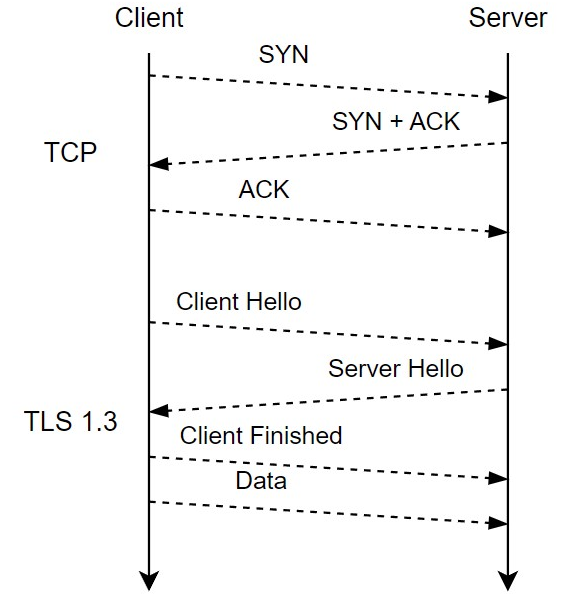
\includegraphics[width=0.7\columnwidth]{descrizione/tcp/tls-handshake}
    \caption{\emph{Processo three-way handshake in TCP con TLS 1.3}}
    \label{tlsHand}
\end{figure}

\noindent I passaggi coinvolti in questo processo sono i seguenti: 
\begin{enumerate}
    \item \textbf{Client invia un messaggio ClientHello al Server}: Il messaggio contiene una lista dei cifrari supportati dal client;
    \item \textbf{Server risponde con un messaggio ServerHello al Client}: Il Server risponde con un messaggio che contiene: 
    \begin{itemize}
        \item  Il cifrario selezionato tra quelli inviati dal Client;
        \item  La chiave pubblica del server per l'algoritmo di scambio chiavi scelto.
    \end{itemize}
    Segue poi il messaggio \emph{Certificate}, che include il certificato del server, e un messaggio \emph{Finished} che conclude la sua parte dell'\emph{handshake};
    \item \textbf{Client invia un messaggio Finished}: Il Client dopo aver ricevuto il messaggio \emph{Finished} dal Server possiede tutte le informazioni necessarie per confermare il completamento dell'\emph{handshake} e invia a sua volta un messaggio \emph{Finished} per confermare il termine di tale operazione.
\end{enumerate}

\noindent È importante notare che con il \emph{TLS 1.3} si ha un \emph{2RTT}, ovvero vengono richiesti due \emph{Round Trip} prima dell'effettivo invio dei dati \cite{site:tls}. 
\subsubsection{UDP (User Datagram Protocol)}
% https://datatracker.ietf.org/doc/html/rfc768
~\\
\indent Dopo aver esaminato il \emph{Transmission Control Protocol (TCP)},
si procede ora all'analisi del \emph{User Datagram Protocol (UDP)}. 
Diversamente dal \emph{TCP}, questo protocollo si distingue come un protocollo senza connessione. 
Questa sua caratteristica significa che non è necessario stabilire una connessione dedicata tra \emph{client} e \emph{server} prima di iniziare lo scambio di dati. 
Questa caratteristica, unita a un \emph{header} di soli 8 \emph{byte} e alla mancanza di un controllo sia di Flusso che di Errore, consente a \emph{UDP} di essere più veloce e leggero rispetto a \emph{TCP}.
\\
Nonostante la sua relativa semplicità, una trattazione esaustiva dell'UDP andrebbe comunque oltre gli scopi di questa tesi. 
Di conseguenza ci si concentrerà sulla struttura di un \emph{datagramma {UDP}} descritto in Figura \ref{udp-datagram}.
\\
\begin{figure}[!h]
    \centering
    \begin{BVerbatim}
 0      7 8     15 16    23 24    31
+--------+--------+--------+--------+
|     Source      |   Destination   |
|      Port       |      Port       |
+--------+--------+--------+--------+
|                 |                 |
|     Length      |    Checksum     |
+--------+--------+--------+--------+
|
|          data octets ...
+---------------- ...
        \end{BVerbatim}
    \caption{\emph{Composizione di un Datagramma UDP}}
    \label{udp-datagram}
\end{figure}

\noindent Si può facilmente notare che l'\emph{header} di un datagramma \emph{UDP} è notevolmente più semplice rispetto a quello di un segmento \emph{TCP}.
In quanto questo è composto da soli quattro campi, i quali sono :  
\begin{itemize}
    \item \textit{\textbf{Source Port - Destination Port}}: Identificano rispettivamente il numero della porta di origine e destinazione. In questo caso il campo relativo alla \emph{source port} può essere omesso ed in tal caso settato a 0.
    \item \textit{\textbf{Lenght}}: Questo campo specifica la lunghezza in byte dell'\emph{header} e del \emph{payload}. La lunghezza minima è di 8 \emph{bytes} mentre il limite superiore è di 65,607 \emph{bytes}.
    \item \textit{\textbf{Checksum}}: Questo campo è opzionale e può essere usato per effettuare dei controli di errore sul datagramma.
\end{itemize}

\noindent La semplicità di questa struttura riflette a pieno i suoi casi d'uso, dove i punti di forza principali sono la velocità e l'efficienza \cite{site:udp}.
In particolare l'assenza di complessi meccanismi di controllo e gestione, invece presenti nel \emph{TCP}, rende l'\emph{UDP} particolarmente adatto per applicazioni che richiedono una trasmissione rapida e in cui la perdita di alcuni pacchetti non invalida totalmente il servizio.
Ne sono un esempio i giochi online, lo streaming video e le chiamate \emph{VOIP}\footnote{\gls{VOIP}}.

\subsection{QUIC}
~\\
\indent I protocolli di trasporto tradizionali come \emph{TCP} e \emph{UDP} hanno servito Internet per decenni, ma nell'era delle comunicazioni moderne, dove le comunicazioni mobili e le applicazioni ad alta velocità dominano le trasmissioni, mostrano alcuni limiti significativi.
\emph{TCP}, nonostante la sua affidabilità, soffre di latenza elevata a causa dell'\emph{overhead} dovuto alla gestione del Flusso. 
Dall'altra parte, \emph{UDP}, pur essendo veloce, manca di meccanismi che ne garantiscono sicurezza e affidabilità.
\\
Sviluppato inizialmente da \emph{Google} nel 2012, \emph{Quic UDP Internet Connections (QUIC)}\footnote{\gls{QUIC}} è stato pensato per affrontare le sfide che i protocolli tradizionali faticavano a gestire, come le performance sulle reti mobili, la sicurezza e la latenza ridotta.
Offrendo una soluzione che combina la velocità dell'\emph{UDP} alla sicurezza e affidabilità del \emph{TCP}. Questo nuovo protocollo si è rapidamente affermato nel mondo delle comunicazioni, tanto da essere standardizzato dall'\emph{IETF}\footnote{\gls{IETF}} nel 2021.
\\\\
Inoltre \emph{QUIC} è stato sviluppato per integrarsi con \emph{HTTP}\footnote{\gls{HTTP}}, chiamando \emph{HTTP/3} la versione che utilizza \emph{QUIC} al posto di
\emph{TCP} come protocollo di trasporto \cite{site:HTTP-over-QUIC} \\\\
\noindent Introduciamo ora gli elementi di \emph{QUIC} che vengono affrontati in questo studio, concentrandoci in particolare su:
\begin{enumerate}
    \item La struttura del protocollo;
    \item Il processo di \emph{handshake};
    \item Multiplexing;
    \item Sistemi di sicurezza;
\end{enumerate}

\subsubsection{Struttura del Protocollo}
~\\ 
\indent Il protocollo \emph{QUIC}, come suggerisce il nome, è costruito sopra al protocollo \emph{UDP}, ovvero tutte le informazioni necessarie al funzionamento di \emph{QUIC} sono contenute nel payload del datagramma \emph{UDP} (Figura \ref{udp-datagram}). 
Questa scelta mira principalmente a evitare l'\emph{ossification}\footnote{\gls{ossification}}, un problema comune nello sviluppo di nuovi protocolli.
L'\emph{ossification} si riferisce alla difficoltà di introdurre nuovi protocolli o modificare quelli esistenti a causa della presenza di dispositivi di rete che si aspettano dei comportamenti specifici dai protocolli conosciuti. Tali dispositivi, noti anche come \emph{middle box}\footnote{\gls{middle box}}, sono gli elementi di rete in cui i pacchetti transitano. 
Costruendo \emph{QUIC} sopra \emph{UDP}, si sfrutta il fatto che l'\emph{UDP} è ampiamente riconosciuto dalle \emph{middle box}, riducendo il rischio che un pacchetto \emph{QUIC} venga scartato. 
Questo approccio permette a \emph{QUIC} di implementare le proprie funzionalità all'interno del payload \emph{UDP}, mantenendo la compatibilità con l'infrastruttura di rete esistente.
\\
Inoltre, l'utilizzo di \emph{UDP} non introduce alcun \emph{overhead}\footnote{\gls{overhead}} significativo e oltre a ciò è già integrato nei vari \emph{sistemi operativi}, cosa che non sarebbe vera se \emph{QUIC} si basasse direttamente su \emph{IP}.
\begin{figure}[!h]
    \centering
    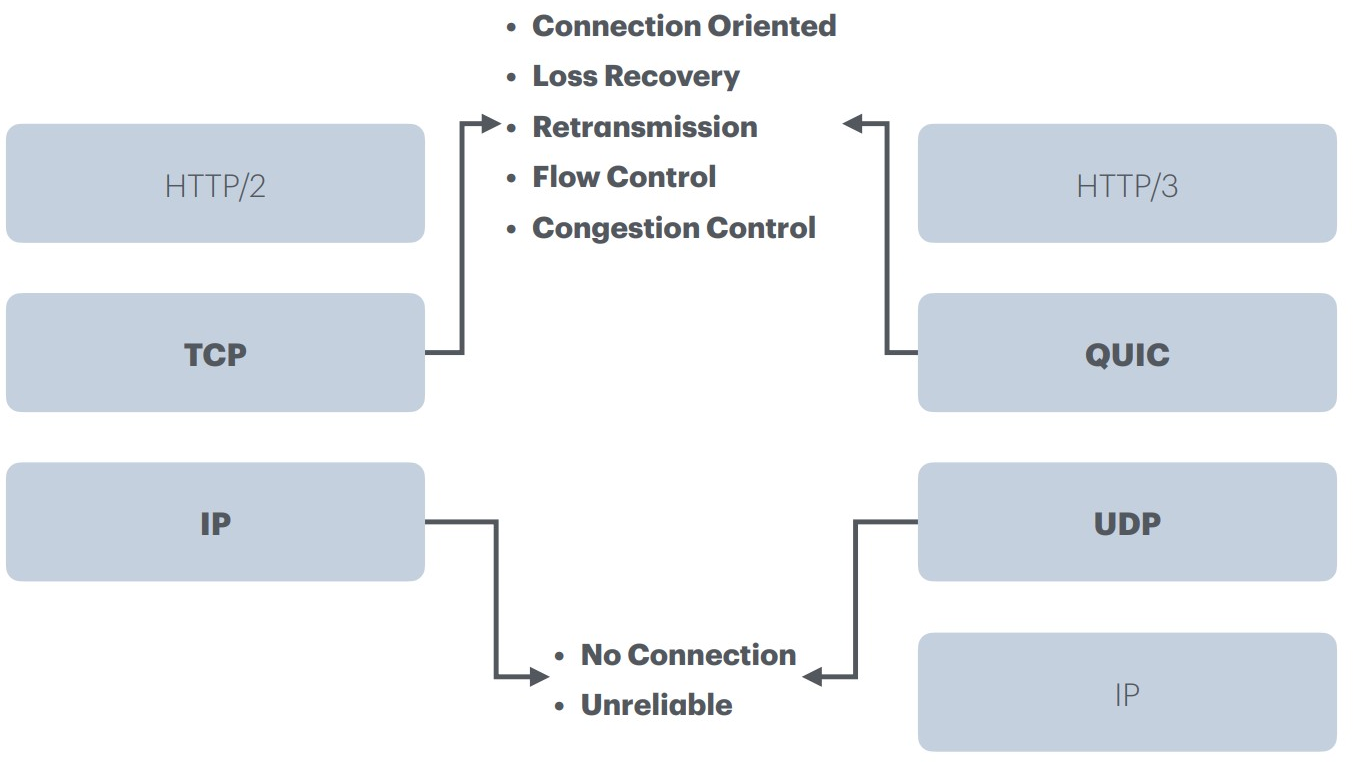
\includegraphics[width=0.7\columnwidth]{descrizione/quic/tcp-quic}
    \caption{\emph{Confronto tra gli stack di protocollo TCP e QUIC}}
    \label{tcp-quic}
\end{figure}
\noindent Come illutrato nella Figura \ref{tcp-quic}, \emph{QUIC} si basa su \emph{UDP} in modo analogo a come \emph{TCP} si basa su \emph{IP}.
Nonostante questa differenza strutturale, \emph{QUIC} implementa le stesse funzionalità chiave di \emph{TCP}, seppur in modo diverso:
\begin{itemize}
    \item Orientato alla connessione;
    \item Recupero delle perdite;
    \item Controllo del flusso;
    \item Ritrasmissione;
    \item Controllo della congestione.
\end{itemize}
\paragraph{\textit{Identificatori di Connessione}}
\noindent A differenza di \emph{TCP}, \emph{QUIC} adotta un approccio diverso per l'identificazione delle connessioni. 
Mentre in \emph{TCP} le connessioni sono identificate tramite la tupla:
\begin{center}
\small
$[\text{Indirizzo IP sorgente}, \text{Porta sorgente}] \leftrightarrow [\text{Indirizzo IP destinazione}, \text{Porta destinazione}]$
\end{center}
\emph{QUIC} introduce un concetto diverso: il \emph{Connection ID}. Questo identificatore consente di riconoscere la connessione in maniera indipendente dagli \emph{indirizzi IP} o dalle \emph{porte} utilizzate.
Il vantaggio principale di questo approccio è la capacità di mantenere attiva una connessione anche in caso di cambiamento dell'\emph{indirizzo IP} o della \emph{porta}, situazione che nelle reti moderne è molto frequente.
\\\\
Un esempio concreto che illustra i vantaggi di questo approccio si può osservare nel comportamento dei dispositivi mobili durante il passaggio tra diverse reti.
Con una connessione \emph{TCP}, quando un dispositivo migra da una rete \emph{WiFi} a una \emph{rete mobile}, è richiesta una riconnessione completa, come si può vedere in Figura \ref{tcp-handoff}. 
\\\\
Al contrario,\emph{QUIC} gestisce questa transazione in modo più efficiente come mostrato nella Figura \ref{quic-handoff}. Grazie al \emph{Connection ID}, \emph{QUIC} riesce a mantenere la connessione attiva nonostante il cambio di rete, eliminando la necessità di effettuare una riconnessione e garantendo un servizio costante \cite{site:Explaining-QUIC}.
\begin{figure}[!h]
    \centering
    \begin{minipage}{0.48\textwidth}
        \centering
        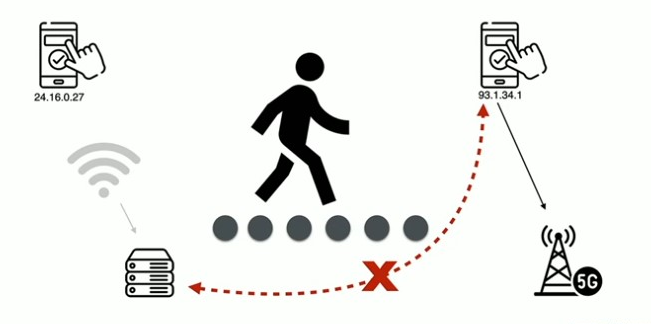
\includegraphics[width=0.90\columnwidth]{descrizione/quic/tcp-handoff}
        \caption{\emph{Meccanismo di hand-off nel caso di connessione TCP}}
        \subcaption*{Con TCP, quando l'utente passa da rete WiFi a rete mobile, ciò comporta un cambiamento del suo indirizzo IP. Tale cambio causa la terminazione della connessione esistente. Poiché TCP identifica la connessione tramite l'indirizzo IP.}
        \label{tcp-handoff}
    \end{minipage}
    \hfill
    \begin{minipage}{0.48\textwidth}
        \centering
        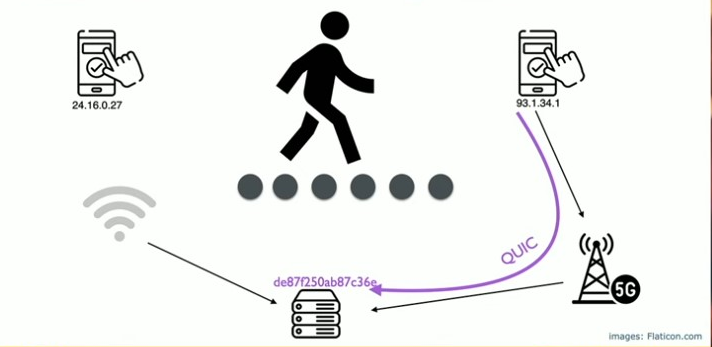
\includegraphics[width=0.90\columnwidth]{descrizione/quic/quic-handoff}
        \caption{\emph{Meccanismo di hand-off nel caso di connessione QUIC}}
        \subcaption*{Con QUIC, quando l'utente passa da WiFi a rete mobile cambiando il suo indirizzo IP, la connessione non viene terminata. Questo perché QUIC utilizza il Connection ID invece dell'indirizzo IP per identificare la connessione, permettendo di mantenere la sessione attiva nonostante il cambio di rete.}
        \label{quic-handoff}
    \end{minipage}
\end{figure}
\\
Oltre a questo vantaggio fondamentale, l'utilizzo del \emph{Connection ID} offre ulteriori benefici:
\begin{itemize}
\item \textbf{Load balancing}: Grazie al \emph{Connection ID} i server possono distribuire il carico in modo più dinamico senza avere interruzioni nelle connessioni esistenti, migliorando le prestazioni e la scalabilità \cite{site:quic-lb}.
\item \textbf{Maggiore privacy}: Il \emph{Connection ID} può essere cambiato frequentemente, aumentando la protezione della privacy e riducendo la tracciabilità delle connessioni \cite{site:quic-security}.
\end{itemize}
\paragraph{\textit{Packet Number}}

\noindent \emph{QUIC} introduce un nuovo meccanismo per la gestione dei numeri di sequenza, ogni pacchetto trasmesso in una connessione \emph{QUIC} viene indentificato tramite un \emph{Packet Number}, un numero univoco 
compreso fra 0 e $2^{62}$-1. Questo numero viene utilizzato per identificare il \emph{nonce crittografico}\footnote{\gls{nonce crittografico}} per la protezione dei pacchetti. 
Per ogni \emph{endpoint}\footnote{\gls{endpoint}} il \emph{Packet Number} è diverso per il traffico in entrata e in uscita. 
Tale dettaglio permette a ciascun \emph{endpoint} di gestire i propri flussi di dati in maniera indipendente, permettendo maggiore flessibilità e sicurezza.
\emph{QUIC}, inoltre, suddivide il \emph{Packet Number} in tre spazi distinti:
\begin{enumerate}[label=\roman*]
    \item \emph{Initial Space}, contiene tutti i pacchetti iniziali.
    \item \emph{Handshake Space}, contiene tutti i pacchetti di \emph{handshake}.
    \item \emph{Application Data Space}, contiene tutti i pacchetti \emph{0-RTT} e \emph{1-RTT}
\end{enumerate}
\noindent Concettualmente, un \emph{packet number space} è il contesto nel quale un pacchetto viene processato e confermato. Questo garantisce che i pacchetti nei \emph{number space} diversi siano crittograficamente separati.
\\
Ogni spazio inizia con un \emph{Packet Number} pari a 0, ogni pacchetto successivo incrementa il numero di 1 alla volta \cite{site:rfc9000}. 

\paragraph{\textit{Formato dei Pacchetti}}
\noindent Un datagramma \emph{UDP} può contenere uno o più pacchetti \emph{QUIC}. Ciascun pacchetto \emph{QUIC} è composto da un \emph{header} e da \emph{N} \emph{frame}, come illustrato nella Figura \ref{quic-packet} secondo le specifiche definite nel RFC 9000 \cite{site:rfc9000}.
\begin{figure}[!h]
    \centering
    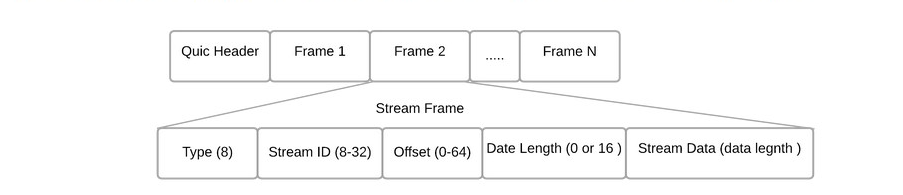
\includegraphics[width=1\columnwidth]{descrizione/quic/packet}
    \caption{\emph{Composizione di un pacchetto QUIC}}
    \label{quic-packet}
\end{figure}
\\
Gli \emph{header} si distinguono in due categorie, \emph{long header} e \emph{short header}. 
\\\\
Il \emph{long header} viene utilizzato principalmente durante la fase di inizializzazione della connessione. 
Di seguito, viene riportata una breve descrizione dei campi presenti (Figura \ref{long-header}) \cite{site:rfc9000}.
\begin{figure}[!h]
    \centering
    \begin{minipage}{0.48\textwidth}
        \centering
        \begin{small}
        \begin{BVerbatim}
 Long Header Packet {
   Header Form (1) = 1,
   Fixed Bit (1) = 1,
   Long Packet Type (2),
   Type-Specific Bits (4),
   Version (32),
   Destination Connection ID Length (8),
   Destination Connection ID (0..160),
   Source Connection ID Length (8),
   Source Connection ID (0..160),
   Type-Specific Payload (..),
 }
        \end{BVerbatim}
    \end{small}
        \caption{\emph{Composizione di un Long Header QUIC}}
        \label{long-header}
    \end{minipage}
    \hfill
    \begin{minipage}{0.48\textwidth}
        \centering
        \begin{tabular}{|c|c|c|}
            \hline
            \textbf{Type} & \textbf{Name}  \\
            \hline
            0x00 & \emph{Initial} \\
            \hline
            0x01 & \emph{0-RTT}  \\
            \hline
            0x02 & \emph{Handshake}   \\
            \hline
            0x03 & \emph{Retry}  \\
            \hline
            \end{tabular}
        \caption{\emph{Tipi di Long Header QUIC}}
        \label{packet-type}
    \end{minipage}
\end{figure}

\begin{itemize}
    \item \textit{\textbf{Header Form}}: 1 bit, indica il tipo di \emph{header}, dove 1 indica \emph{long header}.
    \item \textit{\textbf{Fixed Bit}}: 1 bit, il valore fissato è 1 a meno che non sia un pacchetto di \emph{Negoziazione di Versione}. I pacchetti che contengono 0 in questo campo devono venire scartati.
    \item \textit{\textbf{Long Packet Type}}: 2 bit, specifica il tipo di pacchetto. I tipi di pacchetti sono specificati nella Figura \ref{packet-type}
    \item \textit{\textbf{Type-Specific Bits}}: 4 bit, contiene bit specifici per il tipo di pacchetto.
    \item \textit{\textbf{Version}}: 32 bit, indica la versione di \emph{QUIC} in uso.
    \item \textit{\textbf{Destination Connection ID Length}}: 8 bit, indica la lunghezza del \emph{Connection ID} di destinazione.
    \item \textit{\textbf{Destination Connection ID}}: 0 a 160 bit, indica il \emph{Connection ID} di destinazione.
    \item \textit{\textbf{Source Connection ID Length}}: 8 bit, indica la lunghezza del \emph{Connection ID} di origine.
    \item \textit{\textbf{Source Connection ID}}: 0 a 160 bit, indica il \emph{Connection ID} di origine.
    \item \textit{\textbf{Type-Specific Payload}}: lunghezza variabile, contiene il payload specifico per il tipo di pacchetto.
\end{itemize}

\noindent Una discussione approfondita sui singoli tipi di pacchetto presenti in Figura \ref{packet-type} sarebbe poco inerente motivo per cui si descriverà il ruolo di ogni tipo senza entrare nel dettaglio. 
\\\\
\indent \textbf{\emph{Initial Packet}} ha il compito di trasportare il primo \emph{Crypto Frame} mandato dal \emph{client} e dal \emph{server} per fare lo scambio delle chiavi di crittografia, e si occupa anche di trasportare l'\emph{acknowledge} in entrambe le direzioni.
\\
\indent \textbf{\emph{0-RTT}}  ha il compito di trasportare gli \emph{early data} (dati anticipati) che il \emph{client} invia al \emph{server} come parte della prima comunicazione, questo permette di ridurre la latenza. Si osserverà meglio questo nella sezione dedicata all'\emph{handshake}.
\\
\indent \textbf{\emph{Handshake Packet}}  ha il compito di trasportare i messaggi crittografici necessari per il processo di handshake. Una volta che il \emph{client} ha ricevuto un \emph{Handshake packet} dal \emph{server}, il \emph{client} utilizza pacchetti di \emph{handshake} per inviare i successivi messaggi criptografici di \emph{handshake} e riconoscimenti al \emph{server}.
\\
\indent \textbf{\emph{Retry Packet}}  ha il compito di trasportare un \emph{token} di validazione creato dal \emph{server}. Viene usato dal \emph{server} quando vuole effettuare un \emph{retry}, ovvero richiedere al \emph{client} di ripetere l'invio di una richiesta iniziale.
\\\\
Passiamo ora ad analizzare il \emph{short header}, utilizzato esclusivamente dopo che le chiavi sono state negoziate. Esiste un'unica variante di questo \emph{header}, noto come \emph{RTT-1} (illustrato nella Figura \ref{short-header}) \cite{site:rfc9000}.
\begin{figure}[!h]
    \centering
    \begin{small}
    \begin{BVerbatim}
1-RTT Packet {
    Header Form (1) = 0,
    Fixed Bit (1) = 1,
    Spin Bit (1),
    Reserved Bits (2),
    Key Phase (1),
    Packet Number Length (2),
    Destination Connection ID (0..160),
    Packet Number (8..32),
    Packet Payload (8..),
  }
    \end{BVerbatim}
\end{small}
    \caption{\emph{Composizione di un Short Header QUIC}}
    \label{short-header}
\end{figure}
\begin{itemize}
    \item \textit{\textbf{Header Form}}: 1 bit, indica il tipo di \emph{header}, dove 0 indica \emph{short header}.
    \item \textit{\textbf{Fixed Bit}}: 1 bit, il valore fissato è 1. I pacchetti che contengono 0 in questo campo devono venire scartati.
    \item \textit{\textbf{Spin Bit}}: 1 bit, viene utilizzato per il monitoraggio passivo della latenza, il \emph{server} riflette il valore dello \emph{spin bit} ricevuto mentre il \emph{client} lo inverte dopo ogni \emph{RTT}.
    \item \textit{\textbf{Reserved Bits}}: 2 bit, sono dei bit riservati e protetti usando l'\emph{header protection}, il loro valore dopo aver rimosso la protezione deve essere 0, in caso contrario viene segnalato un errore di connessione.
    \item \textit{\textbf{Key Phase}}: 1 bit, indica la fase della chiave, ovvero permette a chi riceve il pacchetto di identificare le chiavi usate per proteggere il pacchetto. Anche questo campo è protetto usando l'\emph{header protection}.
    \item \textit{\textbf{Packet Number Lenght}}: 2 bit, indica la lunghezza effettiva del campo \emph{Packer Number}
    \item \textit{\textbf{Destination Connection ID}}: 0 a 160 bit, indica il \emph{Connection ID} scelto da chi riceve il pacchetto.
    \item \textit{\textbf{Packet Number}}: 8 a 32 bit, contiene il \emph{Packet Number}.
    \item \textit{\textbf{Packet Payload}}: 8 a lunghezza variabile, contiene il \emph{payload} protetto. 
    \end{itemize}
\subsubsection{Handshake}
Procediamo ora con l'analisi del processo di \emph{handshake} in \emph{QUIC} (Figura \ref{quic-handshake-quic}), evidenziando le differenze rispetto al \emph{handshake} del protocollo \emph{TCP} (Figura \ref{tcp-handshake-quic}).
\begin{figure}[!h]
    \centering
    \begin{minipage}{0.48\textwidth}
        \centering
        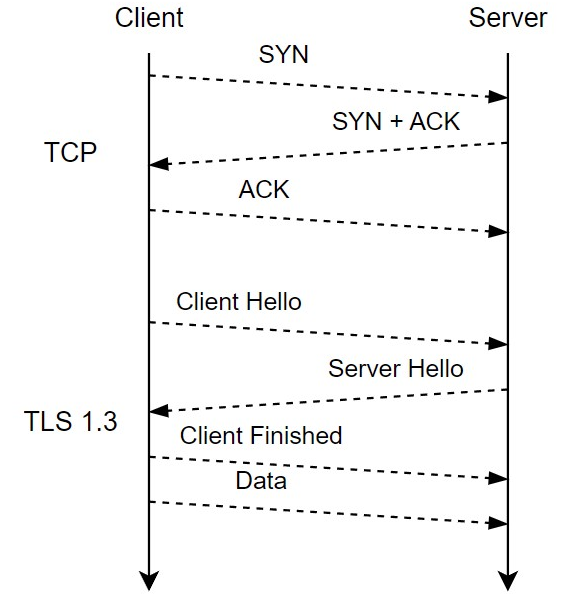
\includegraphics[width=1\columnwidth]{descrizione/tcp/tls-handshake}
        \caption{\emph{Processo three-way handshake in TCP con TLS 1.3}}
        \label{tcp-handshake-quic}
    \end{minipage}
    \hfill
    \begin{minipage}{0.48\textwidth}
        \centering
        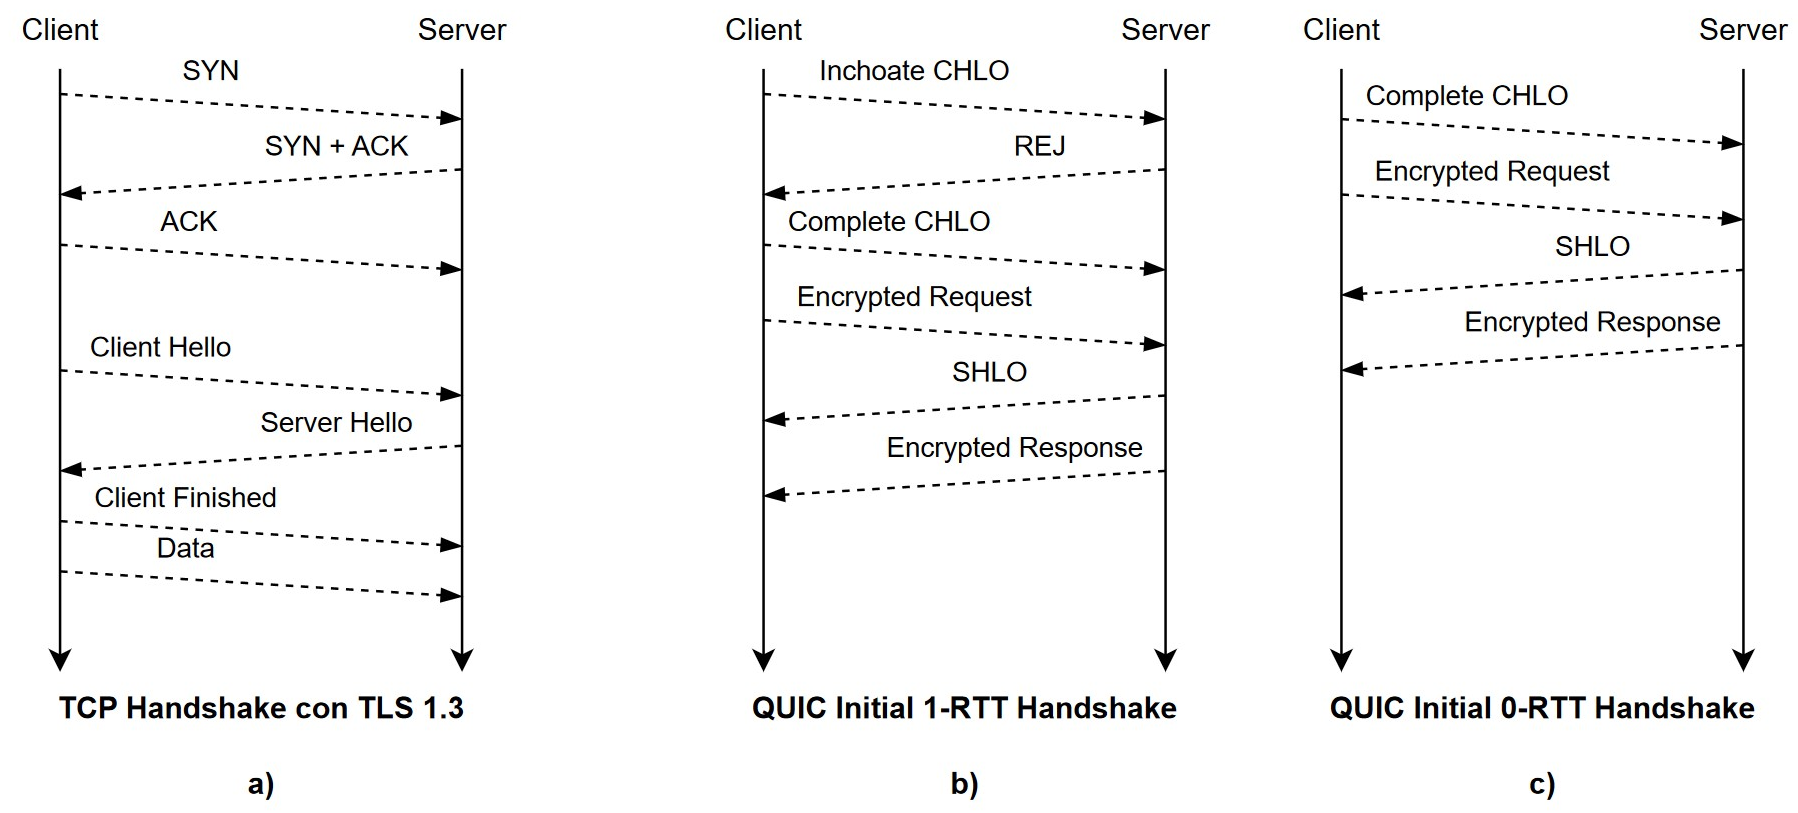
\includegraphics[width=1\columnwidth]{descrizione/quic/handshake}
        \caption{\emph{Processi di handshake in QUIC}}
        \subcaption*{Processo di handshake 1-RTT}
        \subcaption*{Processo di handshake 0-RTT}
        \label{quic-handshake-quic}
    \end{minipage}
\end{figure}

\noindent \emph{QUIC} permette di ridurre significativamente il numero di scambi necessari per l'inizializzazione della connessione rispetto a \emph{TCP}. In particolare, si possono identificare due scenari:
\begin{enumerate}
    \item \textit{\textbf{First-time Connection Establishment}}: Avviene quando il \emph{client} si connette per la prima volta al \emph{server}. Viene inviato un messaggio di \emph{CHLO}\footnote{\gls{CHLO}} a cui il \emph{server} risponde con un messaggio di \emph{REJ}\footnote{\gls{REJ}}. 
    Questo messaggio contiene : 

        \begin{enumerate}[label=\roman*]
            \item La configurazione del server, incluso il valore pubblico di \emph{Diffie-Hellman}\footnote{\gls{Diffie-Hellman}} a lungo termine del server,
            \item Una catena di certificati che autenticano il \emph{server}.
            \item Una firma delle configurazioni del \emph{server} usando una chiave privata presa dal certificato finale della catena.
            \item Un \emph{Source Address Token}, ovvero un blocco di crittografia non autenticata che contiene l'\emph{indirizzo IP} pubblico del \emph{client}.
        \end{enumerate}
        
    Questo token viene utilizzato per verificare l'identità del \emph{client} nelle comunicazioni future. Il \emph{client} usa queste informazioni per autenticare la configurazione del \emph{server} e invia un messaggio \emph{CHLO} completo (\emph{finished}), contenente il valore \emph{Diffie-Hellman} temporaneo del \emph{client} \cite{article:handshake}.
    \item \textit{\textbf{0-RTT Connection Establishment}}: Dopo il primo handshake, il client possiede già le chiavi iniziali per la connessione. Quindi procede con l'invio del \emph{CHLO} completo e può iniziare a inviare dati applicativi al \emph{server}.
    Se l'\emph{handshake} ha successo viene restituito un messaggio \emph{SHLO}\footnote{\gls{SHLO}} cifrato con le chiavi iniziali e contenente il nuovo valore temporaneo di \emph{Diffie-Hellman} \cite{article:handshake}.
\end{enumerate}

\noindent A differenza di \emph{TCP}, che richiede 2 \emph{round trip} per l'invio dei dati dopo l'inizializzazione della connessione, \emph{QUIC} nel caso migliore riesce a ridurre questo numero a 0.

\subsubsection{Multiplexing}
Il \emph{multiplexing} è una tecnica utilizzata nei sistemi di comunicazione per trasmettere più flussi di dati attraverso un singolo canale di comunicazione. 
Tale meccanismo consente di ottimizzare l'uso delle risorse, permettendo a più flussi di dati di condividere la stessa connessione.
\\
In \emph{QUIC}, il \emph{multiplexing} è gestito a livello di \emph{stream}\footnote{\gls{stream}}, permettendo a ogni connessione di ospitare un numero potenzialmente illimitato di \emph{stream} indipendenti.
\\
Ogni \emph{stream} (flusso di dati) è una sequenza ordinata e affidabile di dati che coesiste in parallelo all'interno della stessa connessione. Grazie a questo, la perdita di pacchetti in uno \emph{stream} non interrompe il flusso degli altri, permettendo un utlizzo più efficiente della connessione e migliorando notevolemente le prestazioni in termini di latenza e throughput. Ciò è in contrasto con \emph{TCP}, in cui viene gestita una singola sequenza di dati per connessione.
\\
Un esempio nel quale questo meccanismo risulta particolarmente utile è nelle applicazioni web moderne,
dove spesso vengono richiesti simultaneamente più componenti. 
\\\\
Questo approccio elimina il problema del \emph{Head of Line blocking (HoL)\footnote{\gls{HoL}}}, un fenomeno comune nel \emph{TCP} dove la perdita o il ritardo di un pacchetto obbliga l'intero flusso di dati a interrompersi  finché il pacchetto non viene ritrasmesso e ricevuto correttamente.

\subsubsection{Sicurezza del Protocollo}
Uno degli aspetti fondamentali alla base di \emph{QUIC} è l'attenzione alla sicurezza. Fin dalla sua progettazione iniziale, è stato concepito per migliorare l'affidabilità e la sicurezza delle connessioni. 
Sono diversi i meccanismi integrati all'interno di \emph{QUIC} per ottenere questo obbiettivo.
\\\\
In \emph{QUIC} l'integrazione della sicurezza tramite \emph{TLS 1.3} è parte integrante del protocollo. Il processo di stabilimento della connessione incorpora nello stesso \emph{handshake} la negozazione e l'instaurazione della sicurezza \emph{TLS}. 
Al contrario di \emph{TCP}, dove \emph{TLS} è un protocollo aggiuntivo che viene usato per aggiungere un livello di sicurezza sopra alla connessione \emph{TCP}. Questo comporta molteplici differenze e vantaggi.
\\\\
L'integrazione delle fasi necessarie al \emph{TLS} nel processo di stabilimento della connessione \emph{QUIC} permette di ridurre il numero di round trip necessari.
Inoltre, con \emph{QUIC}, non solo gli \emph{user data} vengono crittografati, ma l'intero pacchetto (\emph{header} escluso) \cite{site:Explaining-QUIC}.
\\\\
Un ulteriore aspetto fondamentale nella sicurezza del protocollo è rappresentato dalla crittografia \emph{end-to-end}\footnote{\gls{end-to-end}}, ciò assicura che i dati trasmessi tra il \emph{client} e il \emph{server} siano protetti da intercettaazioni o manipolazioni da parte di terzi.
Questo avviene tramite l'uso di algoritmi crittografici come \emph{Diffie-Hellman} nella prima fase e successivamente una chiave simmetrica condivisa. Inoltre viene utilizzato un rinnovamento periodico delle chiavi per garantire una maggiore sicurezza e una protezione continua \cite{site:quic-security}.
\\\\
Un altro meccanismo impiegato per garantire l'integrità dei dati è l'utilizzo di un \emph{checksum}, che consente di verificare che i dati non siano stati alterati durante la trasmissione.
Se il destinatario riscotra discrepanze tra il valore del campo \emph{checksum} e i dati stessi, questi verranno rifiutati e scartati.
Inoltre, \emph{QUIC} include nei pacchetti un \emph{hash} crittografico dei dati, che il destinatario può ricalcolare per verificare la presenza di eventuali corruzioni nei dati \cite{site:quic-security}.
\paragraph{\textit{Ritrasmissioni}}
\noindent In seguito viene descritto brevemente il meccanismo di ritrasmissione utilizzato da \emph{QUIC}, che risulta necessario per comprendere alcuni concetti della tesi.
\\\\
In particolare, \emph{QUIC} fa uso di un \emph{Probe TimeOut (PTO)}\footnote{\gls{PTO}} a differenza del \emph{TCP} che invece utilizza il \emph{RTO} tradizionale.
Il \emph{PTO} è un meccanismo progettato per essere più reattivo e flessibile nella gestione delle perdite di pacchetti e nei ritardi.
Questo meccanismo consente di ritrasmettere i pacchetti con un tempo di attesa significativamente ridotto rispetto all'\emph{RTO} tradizionale.
A differenza di quest'ultimo, che aumenta il timeout in modo esponenziale con ogni ritrasmissione fallita, il \emph{PTO} mantiene un intervallo di attesa limitato da una costante massima, migliorando così la reattività e riducendo il tempo per recuperare i pacchetti persi \cite{site:pto-quic}.
\\\\
Viene inoltre usato per gestire separamente i \emph{packet number space} dando priorità ad una fase rispetto ad un'altra. 
Questo garantisce a \emph{QUIC} una maggiore efficienza in reti con alta latenza e perdite di pacchetti.
\subsection{MPTCP}
~\\
\indent \emph{MPTCP} rappresenta un'evoluzione del protocollo \emph{TCP} tradizionale. 
Si tratta di un insieme di estensioni progettate con lo scopo di ampliare le funzionalità del \emph{TCP} standard,
introducendo il concetto di \emph{multipath}\footnote{\gls{multipath}}. Questa innovazione consente a una singola connessione di trasporto di operare simultaneamente su molteplici percorsi di rete.
\\\\
L'idea alla base di \emph{MPTCP} è quella di sfruttare al massimo le varie risorse di rete disponibili, permettendo a una connessione di utlizzare in contemporanea diverse interfacce o percorsi.
\\\\
Questa sezione si focalizzerà primariamente sul funzionamento di \emph{MPTCP}, analizzando i suoi principi base, la struttura del protocollo e i vantaggi che offre rispetto al \emph{TCP} tradizionale. 

\subsubsection{Struttura del Protocollo}
~\\
\indent \emph{Multipath TCP (MPTCP)} introduce una struttura innovativa al livello di trasporto, suddividendolo in due sottolivelli distinti, come illustrato nella Figura \ref{comparison}.
\\\\
Il sottolivello superiore di \emph{MPTCP} opera end-to-end ed è responsabile della gestione complessiva dei vari \emph{subflows} sottostanti. Per fare questo, implementa le seguenti funzioni:
\begin{enumerate}[label=\roman*]
    \item \emph{Path Management}: Gestisce la scoperta, l'aggiunta e la rimozione di percorsi di rete disponibili.
    \item \emph{Packet Scheduling}: Politica con cui si decide in che modo distribuire i pacchetti tra i vari \emph{subflow} attivi.
    \item \emph{Congestion Control}: Implementa un controllo della congestione a livello \emph{MPTCP}, unendo i meccanismi di controllo della congestione dei singoli \emph{subflow}. 
    \item \emph{Subflow Interface}: Si occupa di mappare i dati dell'applicativo sui \emph{subflow} appropriati, gestendo la riordinazione e presentando un flusso di dati coerente all'applicazione.
\end{enumerate}
\noindent Il sottolivello inferiore, è responsabile dei singoli \emph{subflow}. Ogni \emph{subflow} viene trattato come un flusso \emph{TCP} indipendente. Questa struttura permette a \emph{MPTCP} di essere \emph{retro-compatibile} con le reti esistenti, evitando problemi come l'\emph{ossification}. Inoltre, consente al componente \emph{TCP} di operare segmento per segmento, garantendo le funzionalità essenziali del \emph{TCP} tradizionale.
\begin{figure}[!h]
  \centering
    \begin{BVerbatim}
                             +-------------------------------+
                             |           Application         |
+---------------+            +-------------------------------+
|  Application  |            |             MPTCP             |
+---------------+            + - - - - - - - + - - - - - - - +
|      TCP      |            | Subflow (TCP) | Subflow (TCP) |
+---------------+            +-------------------------------+
|      IP       |            |       IP      |      IP       |
+---------------+            +-------------------------------+
        a)                                   b)
               \end{BVerbatim}
    \caption{\emph{Confronto tra gli stack di protocollo TCP e MPTCP standard}}
    \subcaption*{Nel TCP, il protocollo opera su un singolo flusso di dati, utilizzando un unico percorso di rete tra il livello applicazione e lo strato IP.}
    \subcaption*{Con MPTCP, il protocollo gestisce più sottoflussi TCP simultaneamente, permettendo l'utilizzo di percorsi di rete multipli tra il livello applicazione e gli strati IP sottostanti.}
    \label{comparison}
    \end{figure}
\\\\
\noindent Un aspetto fondamentale di questa architettura è la sua trasparenza. Dal punto di vista applicativo, \emph{MPTCP} risulta una singola connessione \emph{TCP} standard, nascondendo la complessità della gestione \emph{multipath} \cite{site:mptcp-design}.
\paragraph{\textit{Formato dei Pacchetti}}
\noindent Essendo una estensione del \emph{TCP} tutte le operazioni del \emph{MPTCP} sono contenute all'interno dei campi opzionali dell'\emph{header TCP}. 
Per identificare le opzioni specifiche di \emph{MPTCP}, il campo \emph{Kind} nell'\emph{header} \emph{TCP} è impostato al valore 30, come assegnato da \emph{IANA}\footnote{\gls{IANA}}.
\begin{figure}[!h]
    \centering
          \begin{BVerbatim}
 1                   2                   3
 0 1 2 3 4 5 6 7 8 9 0 1 2 3 4 5 6 7 8 9 0 1 2 3 4 5 6 7 8 9 0 1
+---------------+---------------+-------+-----------------------+
|     Kind      |    Length     |Subtype|                       |
+---------------+---------------+-------+                       |
|                     Subtype-specific data                     |
|                       (variable length)                       |
+---------------------------------------------------------------+   
        \end{BVerbatim}
    \caption{\emph{Composizione opzione MPTCP}}
    \label{mptcp-option-format}
\end{figure}

\noindent Il campo \emph{Subtype} specifica la funzione dell'opzione \emph{MPTCP}. La Figura \ref{options-subtypes} presenta un elenco completo dei sottotipi disponibili come definito nel RFC 8684 \cite{site:mptcp-packet}. Di seguito, viene riportata una breve descrizione di ogni tipo.

\begin{table}[!h]
    \centering
    \begin{tabular}{|c|c|c|}
        \hline
        \textbf{Value} & \textbf{Symbol} & \textbf{Name} \\
        \hline
        0x0 & \emph{MP\_CAPABLE} & Multipath Capable \\
        \hline
        0x1 & \emph{MP\_JOIN} & Join Connection \\
        \hline
        0x2 & \emph{DSS} & Data Sequence Signal \\
        \hline
        0x3 & \emph{ADD\_ADDR} & Add Address \\
        \hline
        0x4 & \emph{REMOVE\_ADDR} & Remove Address \\
        \hline
        0x5 & \emph{MP\_PRIO} & Change Subflow Priority \\
        \hline
        0x6 & \emph{MP\_FAIL} & Fallback \\
        \hline
        0x7 & \emph{MP\_FASTCLOSE} & Fast Close \\
        \hline
        0x8 & \emph{MP\_TCPRST} & Subflow Reset \\
        \hline
    \end{tabular}
    \caption{\emph{Tabella dei sottotipi dell'opzione MPTCP}}
    \label{options-subtypes}
\end{table}
~\\
\indent \textbf{\emph{Multipath Capable}} viene utilizzato durante il processo di avvio di una connessione, verifica che entrambi gli \emph{endpoint} supportano \emph{MPTCP} e contiene ulteriori informazioni per l'autenticazione di ulteriori \emph{subflow}.
\\
\indent \textbf{\emph{Join Connection}} viene utilizzato per stabilire nuovi \emph{subflow} all'interno di una connessione \emph{MPTCP} esistente, utilizza le informazioni condivise nel \emph{Multipath Capable} per autenticare il \emph{subflow} come parte della connessione principale.
\\
\indent \textbf{\emph{Data Sequence Signal}} gestisce la mappatura dei dati del livello applicativo sui \emph{subflow}, gestendo la riordinazione e la ritrasmissione dei segmenti. 
Utilizza un \emph{Data Sequence Number} a 64 bit per numerare in modo univoco tutti i dati trasmessi attraverso la connessione \emph{MPTCP}.
\\
\indent \textbf{\emph{Add Address}} permette a un \emph{endpoint} di informare la disponibilità di un \emph{indirizzo IP} aggiuntivo disponibile per la connessione, senza stabilire un \emph{subflow}.
\\
\indent \textbf{\emph{Remove Address}} consente a un \emph{endpoint} di notificare che un \emph{indirizzo IP} precedentemente annunciato non è più disponibile.
\\
\indent \textbf{\emph{Change Subflow Priority}} consente di modificare la priorità di un \emph{subflow}, influenzando le decisioni di \emph{Scheduling} del traffico.
\\
\indent \textbf{\emph{Fallback}} segnala la presenza di un problema che richiede il \emph{fallback} al \emph{TCP} normale.
\\
\indent \textbf{\emph{Fast Close}} viene utilizzato per segnalare ad un \emph{endpoint} che la connessione verrà chiusa.
\\
\indent \textbf{\emph{Subflow Reset}} consente di resettare un singolo \emph{subflow} senza influenzare l'intera connessione \emph{MPTCP}.
\\

\indent In conclusione, \emph{MPTCP}, essendo un insieme di estensioni del protocollo \emph{TCP}, ne eredita molte caratteristiche di sicurezza. Questa continuità, offre numerosi vantaggi in termini di compatibilità e robustezza, ma comporta anche alcune problematiche.
\\\\
Da un lato, {MPTCP} utilizza tecniche di sicurezza consolidate come il \emph{three-way-handshake} (opportunamente modificato per gestire il \emph{multipath}) e i meccanismi per il controllo della gestione. 
\\\\
Dall'altra parte, questa stretta dipendenza con \emph{TCP} implica che \emph{MPTCP} sia soggetto a molte delle stesse problematiche e vulnerabilità del \emph{TCP}. 
Inoltre la natura \emph{multipath} del protocollo introduce una nuova possibile superfice d'attacco, richiedendo l'implementazione di meccanismi specifici per autenticare e garantire l'integrità dei singoli \emph{subflow}.

\section{Problematiche Attuali}
\label{Problema}
~\\
\indent Nel contesto delle reti moderne le comunicazioni su reti mobili stanno assumendo un'importanza sempre maggiore, con un numero crescente di dispositivi connessi e un volume di dati in crescita continua. 
La diffusione di smartphone e dispositivi \emph{IoT} ha alimentato un incremento esponenziale del traffico dati, rendendo le reti mobili fondamentali per la la vita quotidiana e per molteplici attività economiche.
In questo contesto, garantire l'efficienza, la sicurezza e la correttezza del traffico dati su queste reti è diventato sempre più una priorità.
\\\\
Un aspetto critico delle reti mobili è la tariffazione del traffico, che spesso si basa sul volume consumato dall'utente. 
Meccanismi di rete come la ritrasmissione dei pacchetti persi possono influenzare questo valore, rendendo complesso il calcolo del consumo. 
Questo comporta che i diversi operatori del traffico cellulare devono decidere che politica adottare per i pacchetti ritrasmessi.
Un primo approccio è quello di addebitare ogni pacchetto per l'utilizzo dell'architettura delle reti mobili. 
Tuttavia, questa politica espone gli utenti a un possibile \emph{Usage-Inflation Attack}, dove un avversario potrebbe aumentare artificialmente il traffico dati ritrasmettendo pacchetti.
Un secondo approccio è quello di escludere i pacchetti ritrasmessi dalla contabilizzazione. Questo scenario, nonostante eviti lo \emph{Usage-Inflation Attack}, aumenta notevolemente la complessità dell'implementazione, richiedendo metodi per il monitoraggio accurato del traffico.
Inoltre, potrebbe essere vulnerabile a \emph{free-riding Attack}, dove gli attaccanti mascherano il proprio traffico all'interno di finti pacchetti ritrasmessi, evadendo così la tariffazione \cite{article:cellular}.
\\\\
Il problema specifico affrontato in questo studio riguarda lo scenario presentato nel primo approccio. L'obiettivo principale della ricerca è stato quello di esplorare eventuali vulnerabilità di \emph{QUIC} che potrebbero essere sfruttate per manipolare i sistemi di contabilizzazione del traffico mobile.
In particolare, lo studio si è concentrato sulle possibili problematiche che causano un aumento della ritrasmissione o eventuali metodi per forzare ritrasmissioni, con lo scopo di aumentare artificialmente la contabilizzazione del traffico.


